\input{../preamble-tmp.tex}

\title%
{Memoria en C++ - Segmentos}

\subject{Memoria en C++ - Segmentos}


\begin{document}

\begin{frame}[noframenumbering,plain]
   \titlepage
\end{frame}

~% macro content() %~
\section{Segmentos de Memoria}
% Stack Heap Data Code
~% if interactive is off %~
\begin{frame}[fragile,label=SM]{Segmentos de memoria}
   \begin{itemize}
      \item<1-> Code segment: de solo lectura y ejecutable, a donde va el c\'odigo y las constantes.
      \item<2-> Data segment: variables creadas al inicio del programa y son v\'alidas hasta que este termina; pueden ser de acceso global o local.
      \item<3-> Stack: variables creadas al inicio de una llamada a una funci\'on y destruidas autom\'aticamente cuando esta llamada termina.
      \item<4-> Heap: variables cuya duraci\'on esta controlada por el programador (run-time).
   \end{itemize}
\end{frame}
~% else %~
\begin{frame}[fragile]{Segmentos de memoria}
   \begin{itemize}
      \item<1-> Code segment: de solo lectura y ejecutable, a donde va el c\'odigo y las constantes.
      \item<2-> Data segment: variables creadas al inicio del programa y son v\'alidas hasta que este termina; pueden ser de acceso global o local.
   \end{itemize}
\end{frame}
\begin{frame}[fragile]{Segmentos de memoria}
   \begin{itemize}
      \item<3-> Stack: variables creadas al inicio de una llamada a una funci\'on y destruidas autom\'aticamente cuando esta llamada termina.
      \item<4-> Heap: variables cuya duraci\'on esta controlada por el programador (run-time).
   \end{itemize}
\end{frame}
~% endif %~
\begin{frame}[fragile,label=LS]{Duraci\'on y visibilidad (lifetime and scope)}
   \begin{itemize}
       \item<1-> Duraci\'on (lifetime): tiempo desde que a la variable se le reserva memoria hasta que esta es liberada. Determinado por el segmento de memoria que se usa.
       \item<2-> Visibilidad (scope): Cuando una variable se la puede acceder y cuando esta oculta.
   \end{itemize}
\end{frame}


% static (variables locales/globales y funciones)
~% if interactive is off %~
\begin{frame}[fragile]{Asignaci\'on del lifetime y scope}
         \begin{lstlisting}[style=dimmided]
@int g = 1;@@
static int l = 1;@@
extern char e;@
@
void Fa() { }@@
static void Fb() { }@@
void Fc();@

void foo(@int arg@) {@
   int a = 1;@@
   static int b = 1;@
   @
   void * p = malloc(4);
   free(p);@
   @
   char *c = "ABC";@@
   char ar[] = "ABC";@
}
         \end{lstlisting}
\end{frame}
\begin{frame}[fragile]{Asignaci\'on del lifetime y scope}
         \begin{lstlisting}[style=normal]
int g = 1;          // Data segment; scope global
static int l = 1;   // Data segment; scope local (este file)
extern char e;      // No asigna memoria (es un nombre)

void Fa() { }        // Code segment; scope global
static void Fb() { } // Code segment; scope local (este file)
void Fc();           // No asigna memoria (es un nombre)

void foo(int arg) {  // Argumentos y retornos son del stack
   int a = 1;        // Stack segment; scope local (func foo)
   static int b = 1; // Data segment; scope local (func foo)

   void * p = malloc(4); // p en el Stack; apunta al Heap
   free(p);              // liberar el bloque explicitamente!!

   char *c = "ABC";   // c en el Stack; apunta al Code Segment
   char ar[] = "ABC"; // es un array con su todo en el Stack
} // fin del scope de foo: las variables locales son liberadas
         \end{lstlisting}
\end{frame}
~% else %~
\begin{frame}[fragile]{Asignaci\'on del lifetime y scope}
         \begin{lstlisting}[style=normal]
int g = 1;
static int l = 1;
extern char e;

void Fa() { }
static void Fb() { }
void Fc();

void foo(int arg) {
   int a = 1;
   static int b = 1;

   void * p = malloc(4);
   free(p);

   char *c = "ABC";
   char ar[] = "ABC";
}
         \end{lstlisting}
\end{frame}
~% endif %~
\note[itemize] {
\item En C++ usaras m\'as frecuentemente \lstinline[style=normal]!new! que \lstinline[style=normal]!malloc! para reservar memoria en el heap. La diferencia es que \lstinline[style=normal]!new! ademas de reservar memoria llama a los constructores (que los veremos pronto).
}

\begin{frame}[fragile]{El donde importa! - Segmentation Fault}
         \begin{lstlisting}[style=normal]

void f() {
   char *a = "ABC";
   char b[] = "ABC";

   b[0] = 'X';
   a[0] = 'X';  // segmentation fault
}
         \end{lstlisting}
\end{frame}
\note[itemize] {
\item Como el puntero "a" apunta al Code Segment y este es de solo lectura, tratar de modificarlo termina en un Segmentation Fault
}

\begin{frame}[fragile]{El donde importa! - Cache friendly}
    \begin{figure}[h]
    \centering
    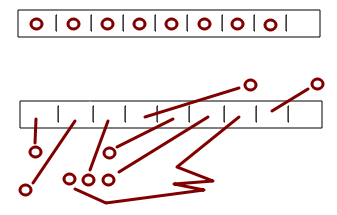
\includegraphics[scale=0.8]{mem_alloc.png}
    \end{figure}
\end{frame}
\note[itemize] {
\item El primer array contiene los elementos de interes mientras que el segundo contiene punteros a los elementos.
\item El array de punteros es m\'as ineficiente (lento) que el primero por 2 razones: hay un nivel de indirecci\'on adicional (hay que dereferenciar el puntero y saltar) y se pierde la localidad.
\item Cuando un valor de memoria es le\'ido, la CPU se trae todo un bloque contiguo de memoria a su cache. Acceder a valores contiguos en memoria es r\'apido por que todos se encuentran en la cache.
\item En cambio, leer valores que estan desperdigados por toda la memoria requiere que el CPU se los traiga de a una a la vez.
\item En la jerga se dice que el primer array es cache friendly.
}


~% endmacro %~

~{ content() }~


\end{document}


